\documentclass{beamer}
\usetheme[hideothersubsections]{HRTheme}
\usepackage{beamerthemeHRTheme}
\usepackage{graphicx}
\usepackage[space]{grffile}
\usepackage{listings}
\lstset{language=SQL,
basicstyle=\ttfamily\footnotesize,
mathescape=true,
keywordstyle=\color{blue},
breaklines=true
showstringspaces=false}
\usepackage[utf8]{inputenc}
\usepackage{color}
\usepackage{wrapfig}
\newcommand{\red}[1]{
\textcolor{red}{#1}
}
\newcommand{\ts}{\textbackslash}
\newcommand{\valseq}[1]{$\lbrace$ #1 $\rbrace$}
\newcommand{\tuple}[2]{$t_{#1}$[#2]}
\newcommand{\fdep}[2]{#1 $\rightarrow$ #2}

\title{Normalization algorithms}

\author{TEAM INFDEV}

\institute{Hogeschool Rotterdam \\ 
	Rotterdam, Netherlands}

\date{}

\begin{document}
\maketitle

\SlideSection{Lesson overview}

\begin{frame}
	\frametitle{Lesson topics}
	\begin{itemize}
		\item Normalization algorithms
		\item Normalization from unnormalized table to 1NF.
		\item Normalization from 1NF to 2NF.
		\item Normalization from 2NF to BCNF.
	\end{itemize}
\end{frame}

\SlideSection{Normalization algorithms}

\begin{frame}
	\frametitle{Normalization algorithms}
	\framesubtitle{Normalization in 1NF}
	
	\begin{itemize}
		\item Find an attribute that is non-atomic, i.e. containing multiple values.
\pause
		\item Remove the non-atomic attribute from the first table creating a new table R1. The primary key of R1 is the primary key of the original relation.
\pause
		\item Create a new table R2 for this attribute. Add the attributes of the primary key of R1 to R2 and all the sub-attributes of the composite attribute. The attributes of the primary key of R1 in R2 are a foreign key to R1.
\pause
		\item The primary key of R2 is a combination of the primary key of R1 and all the sub-attributes having unique values.
\pause
		\item Repeat the procedure for all non-atomic attributes.		
	\end{itemize}
\end{frame}

\begin{frame}
	\frametitle{Normalization algorithms}
	\framesubtitle{Example of normalization in 1NF}
	
	\begin{figure}
		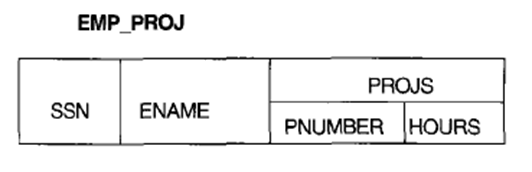
\includegraphics[scale=0.5]{img/normalization/norm14}
	\end{figure}
	
	\begin{itemize}
		\item The composite attribute is PROJS made by the sub-attributes PNUMBER and HOURS.
		\item Create a table EMP\textunderscore PROJ1 containing only SSN (primary key) and ENAME.
		\item Create a table EMP\textunderscore PROJ2 containing SSN,PNUMBER,HOURS. The values of PNUMBER are unique within the composite attribute so the primary key for this table is (SSN,PNUMBER). SSN is a foreign key to EMP\textunderscore PROJ1.	
	\end{itemize}
\end{frame}

\begin{frame}
	\frametitle{Normalization algorithms}
	\framesubtitle{Normalization in 2NF}
	
	\begin{itemize}
		\item Find a non-key attribute that is functionally dependent on a part of the primary key.
\pause
		\item Remove this attribute from the table.
		\item Create a new relation containing this attribute and the subset of the key the attribute is dependent on. The latter will be the primary key of the new table referenced by the same attribute in the first table.
\pause
		\item Repeat the procedure for all the attributes that have a dependency that breaks 2NF.		
	\end{itemize}
\end{frame}

\begin{frame}
	\frametitle{Normalization algorithms}
	\framesubtitle{Example of normalization in 2NF}
	
	\begin{figure}
		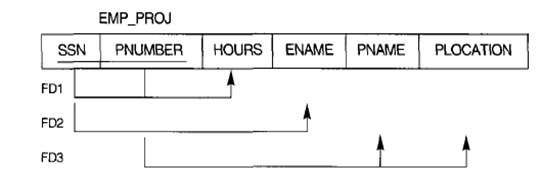
\includegraphics[scale=0.5]{img/normalization/norm15}
	\end{figure}
	
	\begin{itemize}
		\item The dependencies breaking the 2NF are FD2 and FD3.
		\item Remove ENAME,PNAME,PLOCATION from EMP\textunderscore PROJ, creating a new table EP1.
		\item Create a table EP2 containing SSN (primary key) and ENAME.
		\item Create a table EP3 containing PNUMBER (primary key),PNAME,PLOCATION.
		\item In EP1 SSN is a foreign key to EP2 and PNUMBER is a foreign key to EP3.		
	\end{itemize}
\end{frame}

\begin{frame}
	\frametitle{Normalization algorithms}
	\framesubtitle{Example of normalization in 2NF - Result}
	
	\begin{figure}
		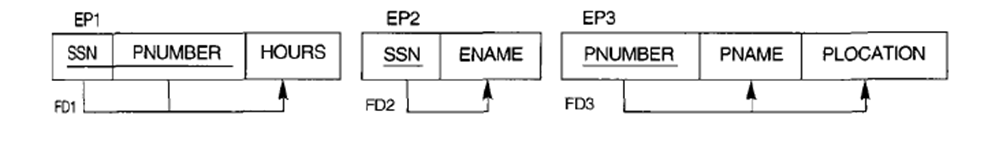
\includegraphics[scale=0.4]{img/normalization/norm16}
	\end{figure}
\end{frame}

\begin{frame}
	\frametitle{Normalization algorithms}
	\framesubtitle{Example of normalization in BCNF}
	
	\begin{itemize}
		\item Find a functional dependency \fdep{X}{A} where X is not superkey of the table.
\pause
		\item Create a new table R1 without A
\pause
		\item Create a new table R2 and add to it X and A. X is the primary key of R2.
\pause
		\item The attribute X in R1 is a foreign key to R2.
	\end{itemize}
	
	\textbf{NOTE:} this normalization algorithm grants the BCNF, which also grants the 3NF. There is another algorithm that grants only the 3NF but with additional properties. We will not see it here.
\end{frame}

\begin{frame}
	\frametitle{Normalization algorithms}
	\framesubtitle{Example of normalization in 3NF/BCNF}
	
	\begin{figure}
		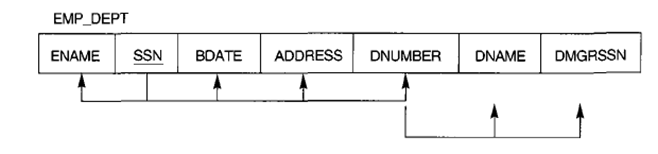
\includegraphics[scale=0.5]{img/normalization/norm17}
	\end{figure}
	
	\begin{itemize}
		\item The dependency breaking the 3NF is \fdep{DNUMBER}{\valseq{DNAME,DMGRSSN}}.
		\item Create a table ED1 containing ENAME,SSN,BDATE,ADDRESS,DNUMBER.
		\item Create a table ED2 containing DNUMBER,DNAME,DMGRSSN.
		\item DNUMBER is the primary key of ED2.
		\item DNUMBER in ED1 is a foreign key to ED2. 
		
	\end{itemize}
\end{frame}

\begin{frame}
	\frametitle{Normalization algorithms}
	\framesubtitle{Example of normalization in 3NF/BCNF - Result}
	
	\begin{figure}
		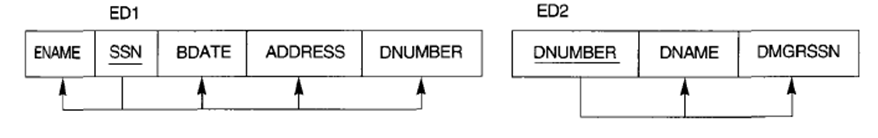
\includegraphics[scale=0.4]{img/normalization/norm18}
	\end{figure}
\end{frame}

\end{document}

\begin{slide}{
\item ...
}\end{slide}

\begin{frame}[fragile]
\begin{lstlisting}
...
\end{lstlisting}
\end{frame}
